% Basic settings
\documentclass[a4paper,10pt]{article}
\usepackage[utf8]{inputenc}
\usepackage[english]{babel}

% Layout settings
\usepackage[top=1.5cm, bottom=1.5cm, left=1.5cm, right=1.5cm]{geometry}
\usepackage[compact]{titlesec}
\titlespacing{\section}{0pt}{0pt}{0pt}
\titlespacing{\subsection}{0pt}{0pt}{0pt}
\titlespacing{\subsubsection}{0pt}{0pt}{0pt}
\setlength{\parindent}{0em}
\setlength{\parskip}{1em}

% Two columns
\usepackage{multicol}

% Package for tables
\usepackage{tabulary,booktabs}

% Colored boxes
\usepackage[most]{tcolorbox}

% package to get colored text
\usepackage{xcolor}

% A base set of colorbox that is then customised
\tcbset {
    base/.style={
        boxrule=0mm,
        leftrule=1mm,
        left=1.75mm,
        arc=0mm,
        fonttitle=\bfseries,
        colbacktitle=black!10!white,
        coltitle=black,
        toptitle=0.75mm,
        bottomtitle=0.25mm,
        title={#1}
    }
}

% Box with red line for definitions
\definecolor{bittersweet}{rgb}{1.0, 0.44, 0.37}
\newtcolorbox{definition}[1]{
    colframe=bittersweet,
    base={#1}
}

% Box with blue line for mainboxes
\definecolor{brandblue}{rgb}{0.34, 0.7, 1}
\newtcolorbox{mainbox}[1]{
    colframe=brandblue,
    base={#1}
}

% Subboxes don't have any color
\newtcolorbox{subbox}[1]{
    colframe=black!20!white,
    base={#1}
}

% Mathematical typesetting & symbols
\usepackage{amsthm, mathtools, amssymb}
\usepackage{amsmath}
\usepackage{amsfonts}
\usepackage{bigints}
\usepackage{mathtools}
\usepackage{wasysym}

% Math helper stuff
\newcommand{\N}{\mathbb{N}}
\newcommand{\Z}{\mathbb{Z}}
\newcommand{\R}{\mathbb{R}}
\newcommand{\Q}{\mathbb{Q}}
\newcommand{\E}{\mathbb{E}}
\newcommand{\F}{\mathbb{F}}
\newcommand{\V}{\mathbb{V}}
\newcommand{\bigO}{\mathcal{O}}
\renewcommand{\d}{\ \mathrm{d}}

% Package to include images/sketches
\usepackage{graphicx}
% Path to graphics
\graphicspath{{images/}}

%###########################################################

\begin{document}
    \section{Funktionen}\label{sec:funktionen}
\setcounter{page}{1}

Für die Beschreibung von Vorgänge, Situationen oder charakteristische Eigenschaften werden zur Darstellung/Modellierung häufig Funktionen benutzt.

\subsection{Einführung}\label{subsec:einfuhrung-funktionen}

\begin{definition}{Funktionen}
    Eine Funktion $f$ ist eine Vorschrift, die jedem Element aus einer Menge $D$ genau ein Element einer Menge $W$ zuordnet.
    Die Menge $D$ wird als \emph{Definitionsbereich} bezeichnet, die Menge $W$ wird als \emph{Wertebereich} bezeichnet.
\end{definition}

\subsection{Darstellungen von Funktionen}\label{subsec:darstellungen-von-funktionen}

Es gibt verschiedene Möglichkeiten, Funktionen darzustellen.
\begin{itemize}
    \item Durch eine Tabelle: $\quad$
    \begin{tabular}{|c|c|c|c|c|c|c|c|c|c|c|}
        \hline
        $x$    & 1 & 2 & 3 & 4  & 5  & 6  & 7  & 8  & 9  & 10 \\
        \hline
        $f(x)$ & 4 & 6 & 8 & 10 & 12 & 14 & 16 & 18 & 20 & 22 \\
        \hline
    \end{tabular}
    \item Durch eine Formel: $y = f(x) = 2x + 2$
    \item Durch einen Graphen:
    \begin{center}
        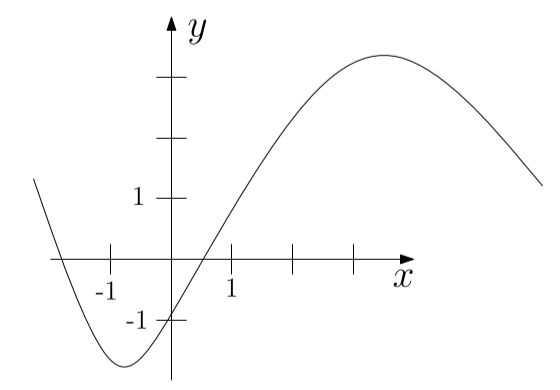
\includegraphics[scale=0.5]{function-graph}
    \end{center}
\end{itemize}

\subsubsection{Nullstellen einer Funktion}

Eine Stelle $x \in D$ mit $f(x) = 0$ heisst \emph{Nullstelle} der Funktion $f$.
Anschaulich ist eine Nullstelle ein Schnittpunkt des Graphen mit der $x$-Achse.
Nullstellen spielen bei vielen Algorithmen, welche zur numerischen Lösung von Gleichungen verwendet werden, eine wichtige Rolle.

\subsection{Operationen mit Funktionen}\label{subsec:operationen-mit-funktionen}

Da die Wertebereiche zweier Funktionen jeweils in $\R$ liegen, lassen sich Funktionen addieren, multiplizieren, etc.
Wir benutzen dieselben Symbole wie bei der Addition, Multiplikation, etc.\ von Zahlen;
streng genommen haben sie hier aber eine andere Bedeutung: Sie beziehen sich auf die Ausführung einer Operation für unendlich viele Werte.

\begin{definition}{}
    Wir betrachten eine beliebige Menge $D$ und zwei Funktionen $f : D \rightarrow \R$ mit $x \mapsto f(x)$ und $g : D \rightarrow \R$ mit $x \mapsto g(x)$.
    Dann können wir die folgenden Operationen definieren:
    \begin{itemize}
        \item Addition: $f + g : D \rightarrow \R$ mit $x \mapsto f(x) + g(x)$
        \item Subtraktion: $f - g : D \rightarrow \R$ mit $x \mapsto f(x) - g(x)$
        \item Multiplikation: $f \cdot g : D \rightarrow \R$ mit $x \mapsto f(x) \cdot g(x)$
        \item Division: $\frac{f}{g} : D \rightarrow \R$ mit $x \mapsto \frac{f(x)} {g(x)} \quad\quad$ falls $g(x) \neq 0$ für alle $x \in D$
        \item Skalierung: $c \cdot f : D \rightarrow \R$ mit $x \mapsto c \cdot f(x) \quad\quad$ für ein fixes $c \in \R$
    \end{itemize}
\end{definition}

\subsection{Komposition}\label{subsec:komposition}

\begin{definition}{Komposition}
    Für zwei gegebene Funktionen $f : A \rightarrow B$ und $g : B \rightarrow C$ ist die Funktion $g \circ f : A \rightarrow C$ definiert durch \[(g \circ f)(x) = g(f(x))\]
    Diese neue Funktion heisst \emph{Komposition} von $f$ und $g$.
\end{definition}

\textbf{Bemerkung:} Zuerst wird die Funktion angewendet, die \emph{rechts} steht!
Ausserdem $f \circ g \neq g \circ f$.

\textbf{Beispiel:} Bestimme die Komposition mit $f(x) = 3x + 7$ und $g(x) = \sqrt{x}$: $(g \circ f)(x) = g(f(x)) = \sqrt{3x + 7}$.

\subsection{Umkehrfunktion}\label{subsec:umkehrfunktion}

\begin{definition}{Umkehrfunktion}
    Eine Funktion $f$ heisst \emph{injektiv}, wenn aus $x_1 \neq x_2$ stets $f(x_1) \neq f(x_2)$ folgt.
    In diesem Fall gibt es für $f$ eine \emph{Umkehrfunktion} $g$ mit \[g(y) \coloneqq x\], wobei $x$ die Eigenschaft $f(x) = y$ hat.
    Sie wird auch mit $f^{-1}$ bezeichnet.
\end{definition}

\textbf{Beispiel:} Bestimme die Umkehrfunktion von $f(x) = \frac{3}{2x-5}$: \[y = \frac{3}{2x-5} \Rightarrow y(2x-5) = 3 \Rightarrow 2xy = 3 + 5y \Rightarrow x = \frac{3 + 5y}{2y} \Rightarrow g(x) = \frac{3+5y}{2y}\]

\subsection{Summenzeichen}\label{subsec:summenzeichen}

Im Zusammenhang mit Funktionen kommt ab und zu das Summenzeichen $\sum$ vor.
Sie ist definiert als \[\sum_{i=1}^n a_i = a_1 + a_2 + \dots + a_n\]

\begin{definition}{Rechenregeln für das Summenzeichen}
    \begin{alignat*}{3}
        &(1) \sum_{k=s}^{n} (c \cdot a_k) &&= c \cdot a_s + c \cdot a_{s+1} + \dots + c \cdot a_n &&= c \cdot \sum_{k=s}^{n} a_K \\
        &(2) \sum_{k=s}^{n} (a_k + b_k) &&= a_s + b_s + a_{s+1} + b_{s+1} + \dots + a_n + b_n &&= \sum_{k=s}^{n} a_k + \sum_{k=s}^{n} b_k \\
        &(3) \sum_{k=s}^{n} a_k + \sum_{k = n + 1}^{m} a_k &&= \sum_{k = s}^{m} a_k = \sum_{r = s}^{m} a_r = \sum_{i = s}^{m} a_i \\
    \end{alignat*}
\end{definition}

\textbf{Bemerkung:} \[\sum_{k=0}^n (a_k \cdot b_k) \neq \left( \sum_{k=0}^n a_k \right) \cdot \left( \sum_{k=0}^n b_k \right)\]

\vspace{-\topsep}

\subsubsection{Spezielle Summenformeln}

\begin{multicols}{2}
    \begin{definition}{Arithmetische Summenformel}
        \[\sum_{k=1}^n k = \frac{n(n+1)}{2}\]
    \end{definition}
    \begin{definition}{Summe der Quadratzahlen}
        \[\sum_{k=1}^n k^2 = \frac{n(n+1)(2n+1)}{6}\]
    \end{definition}
\end{multicols}

    \section{Polynome und weitere elementare Funktionen}\label{sec:polynome}

\begin{definition}{Polynom}
    Eine Polynomfunktion ist eine Funktion der Form: \[y = f(x) = a_n \cdot x^n + a_{n-1} \cdot x^{n-1} + \cdots + a_1 \cdot x + a_0\] mit $a_n \neq 0$, wobei $n$ der \emph{Grad} und $a_0, a_1, \dots, a_n \in \R$ die \emph{Koeffizienten} der Polynomfunktion darstellen.
\end{definition}

\subsection{Das Horner-Schema und der Zerlegungssatz}\label{subsec:horner-schema}

\textbf{Gegeben:} Eine Polynomfunktion $f(x) = a_{n}x^n + a_{n-1}x^{n-1} + \dots + a_{1}x + a_0$.

\textbf{Ziel:} Zu einem gegebenen $x_0$ (z.B. $x_0 = -2$) möglichst effizient den Wert $f(x_0)$ ausrechnen.

\textbf{Variante 1:} Für jedes $k$ den Ausdruck $a_{k}x^{k}$ bestimmen (braucht $k$ Multiplikationen).

$\Rightarrow$ \textbf{Aufwand:} $\quad n + n - 1 + \dots + 2 + 1 + 0 = \frac{n \cdot (n+1)}{2} \quad$
Für $n=10$ werden 55 Multiplikationen benötigt!

\textbf{Variante 2:} Das Horner-Schema verwenden.
Hierbei werden die Terme umgeformt, damit Multiplikation schrittweise erfolgen kann.
Für ein Polynom vom Grad 4:

$\Rightarrow$ \textbf{Aufwand:} $\quad ((((a_4) \cdot x + a_3) \cdot x + a_2) \cdot x + a_1) \cdot x + a_0 \quad$ Anzahl Multiplikationen: 4.

\textbf{Allgemein:} Für ein Polynom vom Grad $n$ werden $n$ Multiplikationen benötigt.
Für $n = 10$ werden also 10 Multiplikation benötigt (statt 55).

\subsubsection{Horner-Schema für Polynom-Auswertung}

Das Schema von Horner biete eine übersichtliche Art, ein Polynom auf diese effiziente Weise auszurechnen.
Veranschaulichung anhand des Beispiels: \[f(x) = 3x^4 - 2x^3 + 5x^2 - 7x - 12\]

\vspace{-\topsep}

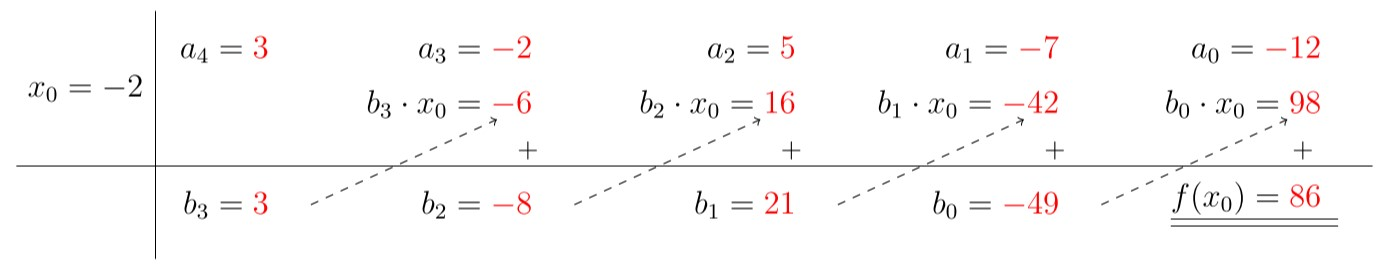
\includegraphics[scale=0.5]{horner-schema}

\subsubsection{Zerlegungssatz}

\begin{definition}{Zerlegungssatz (ohne Beweis)}
    Ist $x_0$ eine Nullstelle der Polynomfunktion $f(x)$, dann gibt es eine bestimmte Polynomfunktion $g(x)$ so dass \[f(x) = (x - x_0) \cdot g(x)\] für jedes x.
\end{definition}

\textbf{Bemerkung:} Der Faktor $(x - x_0)$ heisst Linearfaktor. $g(x)$ ist das sogenannte \emph{1. reduzierte Polynom}: Der Grad von $g(x)$ ist um 1 kleiner als der Grad von $f(x)$.

\subsubsection{Nullstellen von Polynomfunktionen}

\begin{definition}{Satz}
    Eine Polynomfunktion vom Grad $n$ hat höchstens $n$ Nullstellen.
    $x_0$ heisst \emph{m-fache Nullstelle} der Polynomfunktion $f(x)$, falls es eine bestimmte Polynomfunktion $g(x)$ gibt, so dass \[f(x) = (x - x_0)^m \cdot g(x)\] für jedes $x$.
\end{definition}

\subsection{Division von Polynomen}\label{subsec:division-von-polynomen}

Mithilfe des Horner-Schemas können Polynome nur durch \emph{lineare} Faktoren (d.h. Polynome vom Grad 1) dividiert werden.
Zum Beispiel:

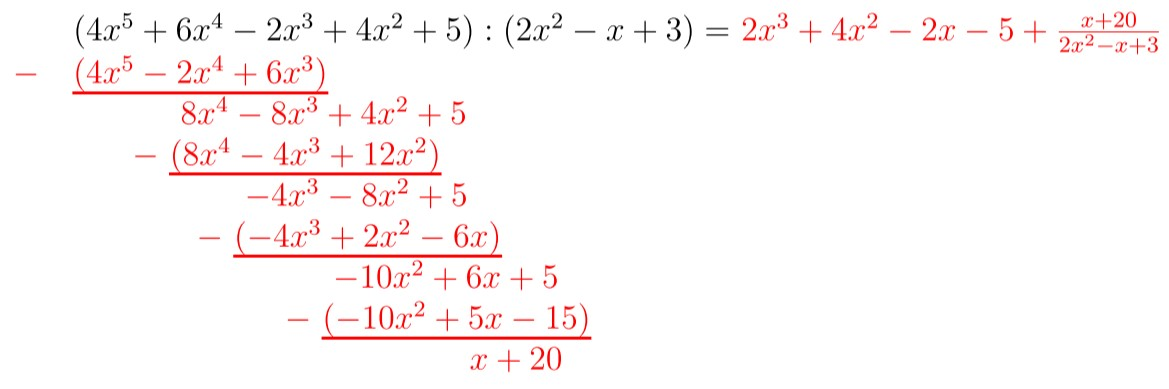
\includegraphics[scale=0.5]{polynom-division}

    \section{Ableitung}\label{sec:ableitung}

\begin{definition}{Definition}
    Die Funktion, die jeder Stelle $x$ den Wert $f'(x)$ zuordnet, wird \emph{Ableitungsfunktion} von $f$ genannt.
    Es werden folgende Schreibweisen verwendet:
    \begin{multicols}{5}
        \begin{itemize}
            \item $f'(x)$
            \item $\frac{\d f}{\d x}$
            \item $\frac{\d y}{\d x}$
        \end{itemize}
    \end{multicols}
\end{definition}

\begin{definition}{Satz}
    Gegeben ist die Funktion $f(x) = c$ mit $c \in \R$.
    Dann gilt: $f'(x) = 0$ für jedes $x \in \R$.
\end{definition}

\textbf{Begründung:} Die Steigung einer horizontalen Geraden ist an jeder Stelle $x$ gleich $0$.

\begin{definition}{Satz}
    Gegeben ist die Funktion $f(x) = x^k$ mit $k \neq 0$.
    Dann gilt: $f'(x) = k \cdot x^{k-1}$.
\end{definition}

\begin{definition}{Ableitung höherer Ordnung}
    Die \emph{zweite Ableitung} erhält man, indem man die Ableitungsfunktion noch einmal ableitet: \[f''(x) = \frac{\d^2 f}{\d x^2} = \frac{\d}{\d x}(f'(x))\]
    Die \emph{dritte Ableitung} erhält man, indem man die zweite Ableitung noch einmal ableitet: \[f'''(x) = \frac{\d^3 f}{\d x^3} = \frac{\d}{\d x}(f''(x))\]
    Und so weiter.
\end{definition}

\textbf{Bemerkung:} Die zweite Ableitung gibt Auskunft über die Veränderung der Ableitung;
wenn man z.B.\ die Geschwindigkeit $v(t)$ ableitet, erhält man die Beschleunigung.

\subsection{Ableitungsregeln}\label{subsec:ableitungsregeln}

\begin{definition}{Faktorregel}
    $(c \cdot f)'(x) = c \cdot f'(x)$
\end{definition}

\textbf{Beispiel:} $(4x^3)' = 4 \cdot (x^3)' = 4 \cdot 3x^2 = 12x^2$

\begin{definition}{Summenregel}
    $(f + g)'(x) = f'(x) + g'(x)$
\end{definition}

\textbf{Beispiel:} $(7x^5 - 3x^3 + 5x^2 - 14x + 6)' = (7x^5)' - (3x^3)' + (5x^2)' - (14x)' + (6)' = 35x^4 - 9x^2 + 10x - 14$

\begin{definition}{Produktregel}
    $(u \cdot v)'(x) = u'(x) \cdot v(x) + u(x) \cdot v'(x)$
\end{definition}

\textbf{Beispiel:} $f(x) = (3x^3 + x^2)(4x^2 + 1)$.
Gesucht ist $f'(x)$.

$u = 3x^3 + x^2$ und $u' = 9x^2 + 2x$\\
$v = 4x^2 + 1$ und $v' = 8x$

$\Rightarrow f'(x) = u'v + uv' = (9x^2 + 2x) \cdot (4x^2 + 1) + (3x^3 + x^2) \cdot 8x = 36x^4 + 9x^2 + 8x^3 + 2x + 24x^4 + 8x^3 = 60x^4 + 16x^3 + 9x^2 + 2x$

\begin{definition}{Quotientenregel}
    $\left( \frac{u}{v} \right)'(x) = \frac{u'(x) \cdot v(x) - u(x) \cdot v'(x)}{(v(x))^2}$
\end{definition}

\begin{definition}{Kettenregel}
    $(F \circ u)'(x) = F'(u) \cdot u'(x)$ wobei
    \begin{itemize}
        \item $F(u)$ die äussere Funktion
        \item $F'(u)$ die Ableitung der äusseren Funktion nach $u$
        \item $u(x)$ die innere Funktion
        \item $u'(x)$ die Ableitung der inneren Funktion nach $x$
    \end{itemize}
    sind.
\end{definition}

\textbf{Beispiel:} $f(x) = (x^3 + 4)^{-2}$

$F(u) = u^{-2}$ und $F'(u) = -2u^{-3}$\\
$u(x) = (x^3 + 4)$ und $u'(x) = 3x^2$

$\Rightarrow f'(x) = -2u^{-3} \cdot 3x^2 = -2(x^3 + 4)^{-3} \cdot 3x^2$

\subsection{Ableitungen bestimmter Funktionen}\label{subsec:ableitungen-bestimmter-funktionen}

\begin{multicols}{2}
    \begin{itemize}
        \item $(\sin (x))' = \cos (x)$
        \item $(\cos (x))' = -\sin (x)$
        \item $(e^x)' = e^x$
        \item $(a^x)' = a^x \cdot \ln (a)$
        \item $(\ln (x))' = \frac{1}{x}$
        \item $(\log_a(x))' = \frac{1}{x \cdot \ln (a)}$
    \end{itemize}
\end{multicols}

\subsection{Differenzierbarkeit}\label{subsec:differenzierbarkeit}

Es gibt Stellen, an denen nur die Funktion, nicht aber die Ableitung definiert ist.
Zum Beispiel ist die Betragsfunktion an der Stelle $x = 0$ nicht differenzierbar.

\begin{definition}{Definition}
    Eine Funktion $f(x)$ ist an der Stelle $x_0$ \emph{differenzierbar}, wenn die linksseitige mit der rechtsseitigen Ableitung übereinstimmt.\\
    Eine Funktion $f(x)$ heisst \emph{differenzierbar} oder \emph{ableitbar}, wenn die Ableitung an jeder Stelle ihres Definitionsbereichs definiert ist.
\end{definition}

    \section{Bestimmtes und unbestimmtes Integral}\label{sec:integral}

Ein Integral $\int_a^b f(x) \d x$ kann man sich als die Fläche unter einem Kurvenstück vorstellen.
\begin{center}
    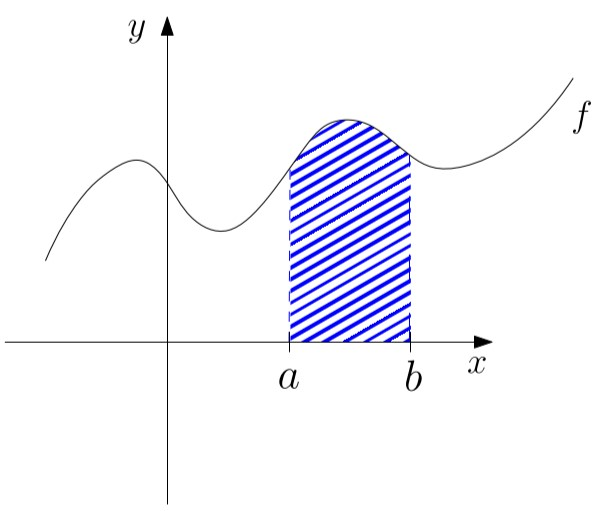
\includegraphics[scale=0.3]{integral}
\end{center}

\subsection{Der Hauptsatz der Differential- und Integralrechnung}\label{subsec:hauptsatz-integralrechnung}

\begin{definition}{Stammfunktionen}
    Gegeben sind ein Intervall $I \subset \R$ und eine Funktion $f : I \rightarrow \R$.
    Eine \emph{Stammfunktion} von $f$ ist eine Funktion $F$, für die gilt: \[F'(x) = f(x)\] für alle $x \in I$.
    D.h.\ wenn man die Stammfunktion ableitet, ergibt sich wieder die Funktion $f$.
\end{definition}

\textbf{Beispiel:} Die Funktion $f(x) = 2x + 1$ hat die Stammfunktionen $F_1(x) = x^2 + x$ und $F_2(x) = x^2 + x + 42$.

Der untenstehende Satz ist Teil vom sogenannten \textbf{Hauptsatz der Differential- und Integralrechnung}.

\begin{definition}{Satz}
    Gegeben ist eine Funktion $f$, die auf einem Intervall $I$ stetig ist, und eine beliebige Stammfunktion $F$ von $f$.
    Dann gilt für alle $a,b \in I$: \[\int_a^b f(x) \d x = F(b) - F(a).\]
\end{definition}

\textbf{Bemerkung:} Das \emph{unbestimmte} Integral $\int f(x) \d x$ bezeichnet eine ``allgemeine'' Stammfunktion der Funktion $f(x)$: \[\int f(x) \d x = F(x) + c\]
Dabei lässt man offen, für welche reelle Zahl die sogenannte \emph{Integrationskonstante} $c$ steht.

\textbf{Achtung:} $\int_a^b f(x) \d x$ ist eine Zahl, $\int f(x) \d x$ ist eine Funktion!

\begin{definition}{Integrationsregeln}
    Gegeben sind zwei Funktion $f$ und $g$ mit Stammfunktionen $F$ bzw. $G$ sowie eine Konstante $c$.
    Dann gilt:
    \begin{enumerate}
        \item $c \cdot F(x)$ ist eine Stammfunktion von $c \cdot f(x)$
        \item $F(x) + G(x)$ ist eine Stammfunktion von $f(x) + g(x)$
    \end{enumerate}
\end{definition}
\begin{definition}{}
    Zusammen mit dem Hauptsatz der Integralrechnung lässt sich daraus folgendes ableiten:
    \begin{enumerate}
        \item $\int_a^b c \cdot f(x) \d x = c \cdot \int_a^b f(x) \d x$
        \item $\int_a^b (f(x) + g(x)) \d x = \int_a^b f(x) \d x + \int_a^b g(x) \d x$
    \end{enumerate}
\end{definition}

\newpage

\textbf{Bemerkung:} Es gibt keine entsprechenden Formeln für Produkte und Quotienten, im Allgemeinen gilt aber: \[\int_a^b (f(x) \cdot g(x)) \d x \neq \left(\int_a^b f(x) \d x\right) \cdot \left(\int_a^b g(x) \d x\right)\] und \[\int_a^b \frac{f(x)}{g(x)} \d x \neq \frac{\int_a^b f(x) \d x}{\int_a^b g(x) \d x}\]

\subsection{Integration von Polynomfunktionen}\label{subsec:integration-polynomfunktionen}

Dank dem Hauptsatz der Differential- und Integralrechnung lässt sich das Integrieren auf das Finden von Stammfunktionen zurückführen.

\textbf{Beispiel 1:} Stammfunktion von $f(x) = c$.

\RIGHTarrow Gesucht ist eine Funktion $F(x)$, sodass $F'(x) = c$.
Die Lösung ist $F(x) = c \cdot x$.

\textbf{Beispiel 2:} Stammfunktion von $f(x) = x^n$ mit $n \in R, n \neq -1$

\RIGHTarrow Gesucht ist eine Funktion $F(x)$, sodass $F'(x) = x^n$.
Die Lösung ist $F(x) = \frac{1}{n + 1} \cdot x^{n + 1}$.

Man kann diese Beispiele verallgemeinern:
\begin{definition}{Satz}
    Für alle $n \in \Z$ mit $n \neq -1$ gilt: \[F(X) = \frac{1}{n + 1} \cdot x^{n + 1}\] ist eine Stammfunktion von $f(x) = x^n$.
\end{definition}

\subsection{Ableitungen und Integrale einiger ausgewählter Funktionen}\label{subsec:ableitungen-und-integrale-funktionen}

\subsubsection*{Potenz- und Logarithmusfunktionen}

\begin{itemize}
    \item $\int a^x \d x = \frac{a^x}{\ln(a)} + C$
    \item $\int \ln(x) \d x = x \cdot \ln(x) - x + C$
    \item $\int \log_a(x) \d x = \frac{1}{\ln(a)} \cdot (x \cdot \ln(x) - x) + C$
\end{itemize}

\subsubsection{Trigonometrische Funktionen}

\begin{itemize}
    \item $\int \sin(x) \d x = -\cos(x) + C$
    \item $\int \cos(x) \d x = \sin(x) + C$
    \item $\int \tan(x) \d x = -\ln |\cos(x)| + C$
    \item $(\tan(x))' = 1 + \tan^2(x) = \frac{1}{\cos^2(x)} \quad$ resp. $\int (1 + \tan^2(x)) \d x = \int \frac{1}{\cos^2(x)} \d x = \tan(x) + C$
    \item $(\arcsin(x))' = (1 - x^2)^{-1/2} \quad$ resp. $\int (1 - x^2)^{-1/2} \d x = \arcsin(x) + C$
    \item $(\arccos(x))' = -(1 - x^2)^{-1/2} \quad$ resp. $\int -(1 - x^2)^{-1/2} \d x = \arccos(x) + C$
    \item $(\arctan(x))' = (1 + x^2)^{-1} \quad$ resp. $\int (1 + x^2)^{-1} \d x = \arctan(x) + C$
\end{itemize}

    \section{Folgen und Reihen}\label{sec:folgen-und-reihen}

\begin{definition}{Definition}
    Eine reelle \emph{Folge} $a$ ist eine Funktion (Abbildung) $a : \N^* \rightarrow \R$, die jeder natürlichen Zahl $n \in \N^*$ eine reelle Zahl $a_n$ zuordnet.

    Indexnotation: $a_n$ ist das $n-te$ Glied der Folge $a$.\\
    Schreibweise: $a = (a_n)$ (oder auch $a = \langle a_n \rangle$).

    Bei einer Folge haben wir es mit unendlich vielen Objekten (reellen Zahlen) zu tun.
\end{definition}

\begin{definition}{Arithmetische Folge}
    Mit $c,d \in \R$
    \begin{itemize}
        \item \textbf{Aufzählende Darstellung:} $c, c + d, c + 2d, c + 3d, \dots$
        \item \textbf{Explizite Darstellung:} $a_n = c + (n - 1)d$
        \item \textbf{Implizite Darstellung:} $a_1 = c$ und $a_{n+1} = a_n + d$
    \end{itemize}
\end{definition}

\begin{definition}{Geometrische Folge}
    Mit $c, q \in \R$ und $q \neq 0,1$
    \begin{itemize}
        \item \textbf{Aufzählende Darstellung:} $c, c \cdot q, c \cdot q^2, c \cdot q^3, \dots$
        \item \textbf{Explizite Darstellung:} $a_n = c \cdot q^{n-1}$
        \item \textbf{Implizite Darstellung:} $a_1 = c$ und $a_{n+1} = a_n \cdot q$
    \end{itemize}
\end{definition}

\begin{definition}{Harmonische Folge}
    \begin{itemize}
        \item \textbf{Aufzählende Darstellung:} $1, \frac{1}{2}, \frac{1}{3}, \frac{1}{4}, \dots$
        \item \textbf{Explizite Darstellung:} $a_n = \frac{1}{n}$
        \item \textbf{Implizite Darstellung:} (Nicht üblich)
    \end{itemize}
\end{definition}

\begin{definition}{Fibonacci-Folge}
    \begin{itemize}
        \item \textbf{Aufzählende Darstellung:} $1, 1, 2, 3, 5, 8, 13, 21, \dots$
        \item \textbf{Explizite Darstellung:} (Nicht elementar)
        \item \textbf{Implizite Darstellung:} $a_1 = 1$, $a_2 = 1$ und $a_{n+2} = a_n + a_{n+1}$
    \end{itemize}
\end{definition}

\subsection{Grenzwerte von Folgen}\label{subsec:grenzwerte-von-folgen}

\begin{definition}{Definition}
    Eine reelle Zahl $g$ heisst \emph{Grenzwert} oder \emph{Limes} der Folge $a_n$, wenn es zu jedem $\epsilon > 0$ eine natürliche Zahl $n_0$ gibt, sodass für alle $n \geq n_0$ stets $|a_n - g| < \epsilon$ gilt.
    Eine Folge heisst \emph{konvergent}, wenn sie einen Grenzwert $g$ hat.
\end{definition}

\begin{center}
    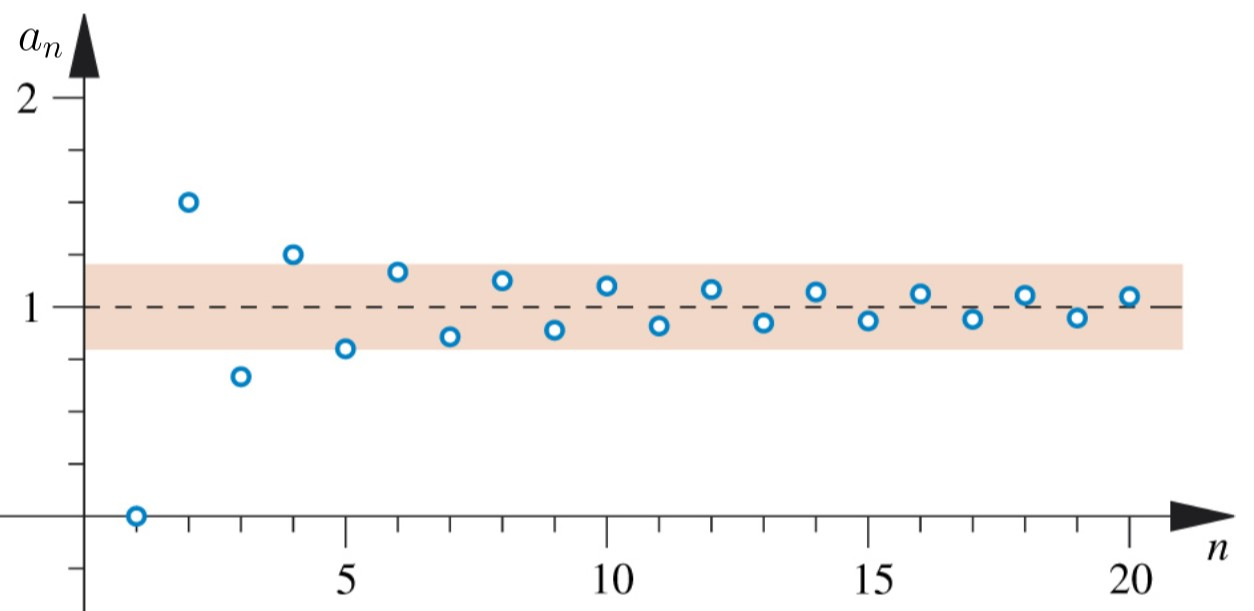
\includegraphics[scale=0.27]{limes}
\end{center}

Damit man sicher sein kann, dass die Punkte immer näher an den geforderten Wert kommen, muss man die Breite des betrachteten Streifens beliebig klein wählen dürfen.
Die Formel dazu lautet: \[g - \epsilon < a_n < g + \epsilon \quad \text{resp.} \quad |a_n - g| < \epsilon\]
Schreibweise: $\lim \limits_{n \rightarrow \infty} a_n = g$.

Eine Folge $a_n$, die keinen Grenzwert hat, heisst \emph{divergent}.

\textbf{Bemerkung:} Eine Folge hat höchstens einen Grenzwert.

\begin{definition}{Rechenregeln für Grenzwerte}
    Gegeben sind zwei konvergente Folgen $a$ und $b$ und eine Konstant $c$.
    Dann gelten:
    \begin{enumerate}
        \item $\lim \limits_{n \rightarrow \infty} (c \cdot a_n) = c \cdot \lim \limits_{n \rightarrow \infty} a_n$
        \item $\lim \limits_{n \rightarrow \infty} (a_n + b_n) = \lim \limits_{n \rightarrow \infty} a_n + \lim \limits_{n \rightarrow \infty} b_n$
        \item $\lim \limits_{n \rightarrow \infty} (a_n - b_n) = \lim \limits_{n \rightarrow \infty} a_n - \lim \limits_{n \rightarrow \infty} b_n$
        \item $\lim \limits_{n \rightarrow \infty} (a_n \cdot b_n) = \lim \limits_{n \rightarrow \infty} a_n \cdot \lim \limits_{n \rightarrow \infty} b_n$
        \item $\lim \limits_{n \rightarrow \infty} \frac{a_n}{b_n} = \frac{\lim \limits_{n \rightarrow \infty} a_n}{\lim \limits_{n \rightarrow \infty} b_n}$, falls $\lim \limits_{n \rightarrow \infty} b_n \neq 0$ und $b_n \neq 0$ für alle $n$.
    \end{enumerate}
\end{definition}

\textbf{Bemerkung:} Wir betrachten eine Folge $a$, die eine rationale Funktion ist, d.h.\ die Folgenglieder sind von der Form $a_n = \frac{g(n)}{h(n)}$, wobei $g(n)$ und $h(n)$ Polynome sind.
Dann wird der Grenzwert $\lim \limits_{n \rightarrow \infty} a_n$ so bestimmt:
\begin{enumerate}
    \item Der Bruch wird mit der höchsten Potenz von $n$, die vorkommt, gekürzt.
    \item Nun wird das Verhalten der einzelnen Summanden für $n \rightarrow \infty$ untersucht.
    \item Daraus kann man den gesuchten Grenzwert bestimmen.
\end{enumerate}
\textbf{Folgerung:} Um den Grenzwert für $n \rightarrow \infty$ zu bestimmen, reicht es, den \emph{höchsten} Exponenten im Zähler und den höchsten Exponenten im Nenner zu betrachten.
Es gibt drei mögliche Fälle:
\begin{itemize}
    \item[] \textbf{Fall 1:} Zählergrad $<$ Nennergrad.
    Dann gilt: $\lim \limits_{n \rightarrow \infty} \frac{g(n)}{h(n)} = 0$\\
    Beispiel: $\lim \limits_{n \rightarrow \infty} \frac{3n^2 + 7n - 15}{n^3 - 2n^2 + n + 10} = 0$
    \item[] \textbf{Fall 2:} Zählergrad $>$ Nennergrad.
    Dann gilt: $\frac{g(n)}{h(n)} \rightarrow \infty$ oder ($-\infty$)\\
    Beispiel: $\frac{3n^4 + 7n - 15}{6n^3 - 2n^2 + 10} \rightarrow \infty$
    \item[] \textbf{Fall 3:} Zählergrad $=$ Nennergrad.
    Dann gilt: $\lim \limits_{n \rightarrow \infty} \frac{g(n)}{h(n)} = \frac{\text{``Führender Term von $g$''}}{\text{``Führender Term von $h$''}}$\\
    Beispiel: $\lim \limits_{n \rightarrow \infty} \frac{2n^3 + n^2 + 8n}{5n^3 + 4n^2 + 17} = \frac{2}{5}$
\end{itemize}

\textbf{Bemerkung:} Die spezielle Folge $\langle \left(1 + \frac{1}{n}\right)^n \rangle$ strebt gegen $e \approx 2.718$.

\subsection{Reihen - einige besondere Beispiele}\label{subsec:reihen-beispiele}

\begin{definition}{Definition}
    Die \emph{Summenfolge} oder \emph{Reihe} $s$ der reelle Folge $a$ ist definiert durch:
    \begin{align*}
        s_1 &= a_1 \\
        s_2 &= a_1 + a_2 \\
        s_3 &= a_1 + a_2 + a_3 \\
        &\vdots \\
        s_n &= a_1 + a_2 + \dots + a_n = \sum \limits_{k=1}^n a_k
    \end{align*}
    Auch ``$n$-te Teilsumme'' genannt.
\end{definition}

\begin{definition}{Arithmetische Reihe}
    Bei einer \emph{arithmetischen Folge} ist die Differenz zweier aufeinanderfolgender Glieder konstant:\\ $a_k - a_{k-1} = d$ für jedes $k$.
    Die Summe der ersten $n$ Glieder einer arithmetischen Folge ist: \[s_n = n \cdot a_1 + \frac{n(n-1)}{2} \cdot d\]
\end{definition}

\begin{definition}{Geometrische Reihe}
    Bei einer \emph{geometrischen Folge} ist der Quotient zweier aufeinanderfolgender Glieder konstant:\\ $\frac{a_k}{a_{k-1}} = q$ für jedes $k$ (mit $q \neq 0, 1$).
    Die Summe der ersten $n$ Elemente einer geometrischen Reihe ist: \[s_n = \frac{a_1 (q^n - 1)}{q - 1} = \frac{a_1 (1 - q^n)}{1 - q}\]
\end{definition}

\subsection{Grenzwerte von Reihen}\label{subsec:grenzwerte-reihen}

Für den Grenzwert der Reihe $s$ einer reellen Folge $a$ schreiben wir: $g = \lim \limits_{n \rightarrow \infty} s_n = \sum_{k=1}^\infty a_k$

% TODO: Andere Reihen auflisten

\textbf{Allgemein (Geometrische Reihe):} Wie verhält sich $s_n = a_1 \cdot \frac{1-q^n}{1-q}$, wenn $n \rightarrow \infty$?
\begin{itemize}
    \item[] \textbf{Fall 1:} $q > 1$.
    Die Reihe strebt gegen $\infty$ oder $-\infty \rightarrow$ Sie hat keinen Grenzwert.
    \item[] \textbf{Fall 2:} $q \leq -1$.
    Die Reihe sprint zwischen positiven und negativen Werten hin und her $\rightarrow$ Sie hat keinen Grenzwert.
    \item[] \textbf{Fall 3:} $|q| < 1$.
    Die Reihe strebt gegen den Grenzwert $a_1 \cdot \frac{1}{1-q}$.
\end{itemize}

\begin{definition}{Zusammenfassung}
    Eine geometrische Reihe konvergiert genau dann, wenn $|q| < 1$ ist.
    Der Grenzwert ist dann $\frac{a_1}{1-q}$.
\end{definition}

    \section{Grenzwerte und Stetigkeit einer Funktion}\label{sec:grenzwerte-und-stetigkeit}

\subsection{Grenzwert einer Funktion im Endlichen}\label{subsec:grenzwert-funktion-im-endlichen}

\begin{definition}{Definition}
    Wir betrachten eine Funktion $f(x)$ und eine Stelle $x_0$.
    Dann bezeichnet der \emph{Grenzwert} $g$ von $f(x)$ an der Stelle $x_0$ denjenigen Wert, dem sich die Funktion annähert, wenn $x$ immer mehr gegen $x_{0}$ geht.

    Wir schreiben dies als $\lim \limits_{x \rightarrow x_0} f(x) = g$ oder $f(x) \rightarrow g$ für $x \rightarrow x_0$.
\end{definition}

\textbf{Bemerkung:} Es ist nicht notwendig, dass die Funktion $f$ an der Stelle $x_0$ definiert ist.

\begin{definition}{Rechenregeln für Grenzwerte}
    \begin{itemize}
        \item $\lim \limits_{x \rightarrow x_0} (c \cdot f(x)) = c \cdot \left( \lim \limits_{x \rightarrow x_0} f(x) \right)$ für $c \in \R$.
        \item $\lim \limits_{x \rightarrow x_0} (f(x) + g(x)) = \lim \limits_{x \rightarrow x_0} f(x) + \lim \limits_{x \rightarrow x_0} g(x)$.
        \item $\lim \limits_{x \rightarrow x_0} (f(x) - g(x)) = \lim \limits_{x \rightarrow x_0} f(x) - \lim \limits_{x \rightarrow x_0} g(x)$.
        \item $\lim \limits_{x \rightarrow x_0} (f(x) \cdot g(x)) = \left( \lim \limits_{x \rightarrow x_0} f(x) \right) \cdot \left( \lim \limits_{x \rightarrow x_0} g(x) \right)$.
        \item $\lim \limits_{x \rightarrow x_0} \frac{f(x)}{g(x)} = \frac{\lim \limits_{x \rightarrow x_0} f(x)}{\lim \limits_{x \rightarrow x_0} g(x)}$ mit der Voraussetzung, dass $\lim \limits_{x \rightarrow x_0} g(x) \neq 0$.
    \end{itemize}
\end{definition}

\subsection{Grenzwerte von gebrochenrationalen Funktionen}\label{subsec:grenzwerte-gebrochenrationalen-funktionen}

\subsection{Grenzwert einer Funktion im Unendlichen}\label{subsec:grenzwert-funktion-im-unendlichen}

\begin{definition}{Definition}
    Der Grenzwert $g$ einer Funktion $f(x)$ im Unendlichen bezeichnet denjenigen Wert, dem sich die Funktion annähert, wenn $x$ gegen unendlich geht.\\

    Schreibweise: $\lim \limits_{x \rightarrow \infty} f(x) = g$\\
    Analog: $f(x) \underset{x \rightarrow\infty}{\longrightarrow} g$
\end{definition}

\textbf{Beispiel:} $\lim \limits_{x \rightarrow \infty} \frac{x}{1 + x^2} = 0$

\RIGHTarrow Begründung: Nennergrad $>$ Zählergrad, daher konvergiert die Funktion gegen 0.

\subsection{Stetigkeit von Funktionen}\label{subsec:stetigkeit}

\begin{definition}{Definition}
    Eine Funktion $f(x)$ heisst \emph{stetig an der Stelle $x_0$}, wenn der Grenzwert $\lim \limits{x \rightarrow x_0} f(x)$ existiert und gleich $f(x_0)$ ist.
\end{definition}

\begin{definition}{Definition}
    Eine Funktion $f(x)$ heisst \emph{stetig}, wenn sie an jeder Stelle ihres Definitionsbereichs stetig ist.
\end{definition}

\textbf{Einfache Vorstellung:} Eine Funktion ist auf einem Intervall $I$ stetig, wenn sich ihr Graph in einem Zug, ohne Absetzen, zeichnen lässt.

\textbf{Bemerkung:} Viele Funktionen, die in der Praxis vorkommen, sind in ihrem Definitionsbereich stetig:
\begin{itemize}
    \item Polynomfunktionen
    \item Rationale Funktionen
    \item Trigonometrische Funktionen ($\tan(x)$, $\sin(x)$, $\cos(x)$)
    \item Exponential- und Logarithmusfunktionen
    \item Potenzfunktionen, Wurzelfunktionen
\end{itemize}

\begin{definition}{Satz}
    Die Summe, die Differenz, das Produkt und die Komposition von stetigen Funktionen sind stetig.
\end{definition}

\begin{definition}{Satz}
    Falls eine Funktion $f(x)$ auf einem Intervall $\left[a,b\right]$ stetig ist, und $f(a)$ und $f(b)$ verschiedene Vorzeichen haben, dann hat $f$ in diesem Intervall mindestens eine Nullstelle.
\end{definition}

    %\section{Kurvendiskussion}\label{sec:kurvendiskussion}

\begin{center}
    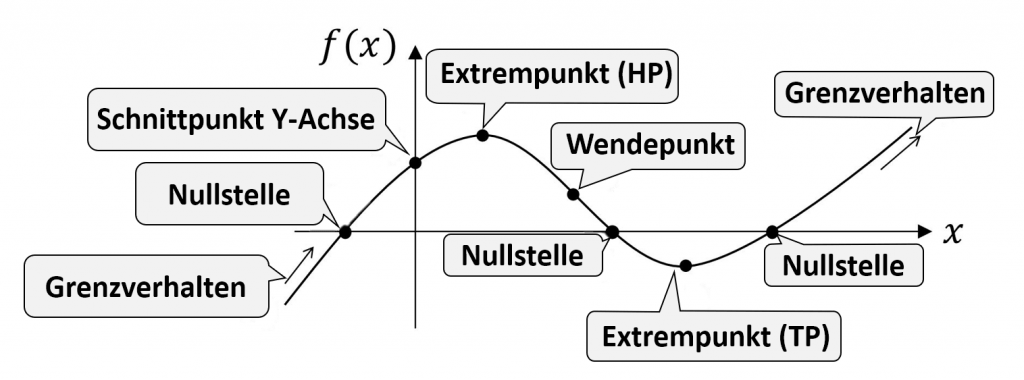
\includegraphics[scale=0.3]{kurvendiskussion}
\end{center}

\begin{definition}{Fragenkatalog für die Kurvendiskussion}
    \begin{enumerate}
        \item Definitionsbereich?
        \item Symmetrieeigenschaften (Gerade, ungerade, periode)?
        \item Schnittpunkte mit Achsen, Polstellen?
        \item Randpunkte bzw.\ Verhalten, wenn $x$ gegen die Grenzen des Definitionsbereichs strebt?
        \item Kandidaten für Extrema bestimmen und untersuchen
        \item Wendepunkte suchen
        \item Tabelle von Werten aufstellen (falls nötig)
    \end{enumerate}
\end{definition}

\end{document}